%! Author = noone
%! Date = 9/10/22

% Preamble
\documentclass[11pt]{article}

% Packages
\usepackage{amsmath}
\usepackage{graphicx}
\usepackage{amsfonts}
\usepackage{float}

% Document
\begin{document}

\part{Reinforcement Learning}\label{part:reinforcement-learning}

\section{Purpose}\label{sec:purpose}
The topic for this week is Reinforcement Learning (RL).
We will see how reinforcement learning tasks can be formally defined, compare
different models of optimality, and discuss the need for exploration and the
problem of delayed rewards.
We will present a number of RL algorithms including Temporal Difference
learning (TD-learning), Q-learning, policy gradients, actor-critic.
We will see how RL can be applied to games like backgammon, and how deep
Q-learning or A3C can learn to play Atari games from raw pixels.

\subsection{Activity Instructions}\label{subsec:activity-instructions}
Complete the exercises (both non-coding and coding) in Ed to help you check
your understanding and prepare for your assessments.

\section{Week 5: Overview}\label{sec:week-5:-overview}
The topic for this week is Reinforcement Learning (RL).
We will see how reinforcement learning tasks can be formally defined, compare
different models of optimality, and discuss the need for exploration and the
roblem of delayed rewards.
We will present a number of RL algorithms including Temporal Difference
learning (TD-learning), Q-learning, policy gradients, actor-critic.
We will see how RL can be applied to games like backgammon, and how deep
Q-learning or A3C can learn to play Atari games from raw pixels.

\subsection{Weekly learning outcomes}\label{subsec:weekly-learning-outcomes}
By the end of this week, you will be able to:

\begin{enumerate}
  \item explain the difference between supervised learning, reinforcement learning, and unsupervised learning
  \item describe the formal definition of a reinforcement learning task
  \item identify different models of optimality
  \item explain the need for exploration in reinforcement learning
  \item describe reinforcement learning algorithms, including TD-learning, Q-learning, policy gradients, and actor-critic
  \item apply Q-learning to simple tasks.
\end{enumerate}

\subsection{Reinforcement Learning}\label{subsec:reinforcement-learning}
We have previously discussed supervised learning, where pairs of inputs and
target outputs are provided and the system must learn to predict the correct
output for each input.

There are many situations where we instead want to train a system to perform
certain actions in an environment, in order to maximise a reward function.
These situations include, for example, playing a video game, allocating mobile
phone channels or other resources dynamically, driving a car or flying a
helicopter.

Supervised learning can sometimes be used for this purpose, if we construct a
training set of situation-action pairs (for example, a database of game
positions and the move chosen by a human expert, or sensor readings from a
motor car and the steering direction chosen by a human driver).
This process is sometimes called Behavioral Cloning.

However, it is often better if the system can learn by purely by self-play,
without the need for training data from a human expert.

\subsection{Reinforcement Learning Framework}\label{subsec:reinforcement-learning-framework}
Reinforcement Learning (RL) can be formalised in terms of an Agent interacting
with its Environment.

The Environment includes a set of $S$ states and a set of $A$ actions.
At each time step $t$, the agent is in some state $s_t$.
It must choose an action $a_t$, whereupon it goes into state
$s_{t + 1} = \delta (s_t , a_t)$ and receives reward $r_t = R(s_t, a_t)$

The Agent chooses its actions according to some
\textbb{policy} $\pi : S \rightarrow A $

The aim of Reinforcement Learning is to find an \textbb{optimal} policy which
maximises the cumulative reward.

In some cases, the Environment may be probabilistic or \textbb{stochastic} −−
meaning that the transitions and/or rewards are not fully determined, but
instead occur randomly according to some probability distribution:
\[\delta (s_{t = 1} = s | s_t, a_t),R (r_t = r | s_t, a_t)\]

The Agent can also employ a probabilistic policy, with its actions chosen
according to a probability distribution:

\[\pi (a_t = a | s_t)\]

\subsection{Optional Video}\label{subsec:optional-video}
insert video

\subsection{Probabilistic Policies}\label{subsec:probabilistic-policies}
The main benefit of a probabilistic policy is that it forces the agent to
explore its environment more comprehensively while it is learning.

However, probabilistic policies may have additional benefits in other contexts,
such as partially observable or multiplayer environments.

\begin{figure}[h]
    \centering
    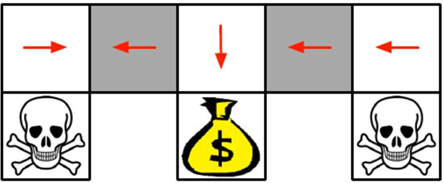
\includegraphics[width=\textwidth]{../out/images/probabilistic-policy}
    \caption[probabilistic policy]{probabilistic policy}
    \label{fig:probabilistic policy}
\end{figure}

Consider, for example, a situation in which the Agent is able to observe that
it is in one of the grey squares, but is not able to determine which grey
square it is in.
In this case, the policy of moving left or right with equal probability from
the grey square will perform better than any deterministic policy.

In two-player games like rock-paper-scissors, a random strategy is also
required in order to make agent choices unpredictable to the opponent.

\subsection{Optional video}\label{subsec:optional-video2}
insert video

\subsection{Models of Optimality}\label{subsec:models-of-optimality}
What exactly do we mean when we say that an RL Agent should choose a policy
which maximises its future rewards?

The old saying \("\)a fast nickel is worth a slow dime\("\) reminds us that people
often prefer to receive a smaller reward sooner instead of a larger reward
later.
Economists use surveys to gauge people's preferences in this regard: \("\)Would
you prefer ten dollars today, or 15 dollars next week?
How about 50 dollars today compared to 100 dollars next year?\("\) Responses
to these surveys can be used to estimate a number $gamma$ between $0$ and $1$
that is chosen such that one dollar in the current timestep is considered
equally desirable with $gamma$ dollars in the next timestep.
In Reinforcement Learning, this number $gamma$ is called the discount factor
and is used to define the infinite discounted reward, which can be compared
with average reward and finite horizon reward.

\[
\begin{aligned}
    \text{Finite horizon reward} &: \sum_{i=0}^{h-1} r_{t+1} \\
    \text{Infinite discounted reward} &: \sum_{i=0}^{\infty} \gamma^i r_{t+i}, 0 \leq \gamma \leq 1\\
    \text{Average Reward} &: \lim_{h \to \infty} \dfrac{1}{h} \sum_{i=0}^{h-1} r_{t+1} \\
\end{aligned}
\]

We normally try to maximise the infinite discounted reward, because it is
easier to analyse theoretically and also works well in practice.

The finite horizon reward is easy to compute, but may lead to bad decisions by
failing to take into account rewards which are just over the horizon.

 Average reward is hard to deal with because we cannot sensibly choose between
a small reward soon and a large reward very far in the future −-− for example,
100 dollars today compared with a million dollars, 50 years from now.

\subsection{Comparing Models of Optimality}\label{subsec:comparing-models-of-optimality}

\begin{figure}[h]
    \centering
    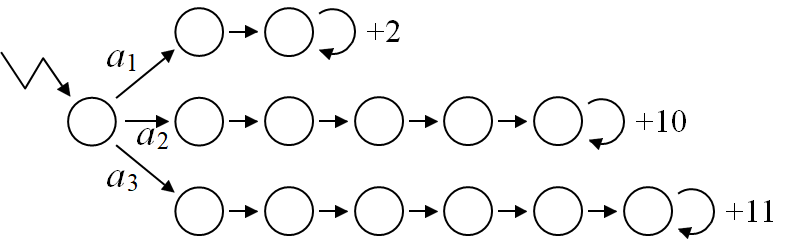
\includegraphics[width=\textwidth]{../out/images/comparing-models-of-optimality}
    \caption[comparing models of optimality]{comparing models of optimality}
    \label{fig:comparing models of optimality}
\end{figure}

This environment illustrates how the choice of action may depend on the model
of optimality.
An agent trying to maximise the finite horizon reword with $h=4$ would prefer
action $a_1$ because it is the only action which will gain any reward within
the first four time steps.
An agent maximising average reward will prefer action $a_3$ because, after the
first few time steps, it will be getting a reward of +11 every timestep which
is larger than +10 for an agent who chose action $a_2$.
An agent maximising infinite discounted reward with $\gamma=0.9$ will prefer
action $a_2$.
One way to see this is as follows: Consider Agent $A_2$ choosing action $a_2$,
compared to Agent $A_3$ choosing action $a_3$.
The reward of 11 received by $A_3$ in timestep 7 would be equivalent to 9.9 in
timestep 6 and therefore slightly less than the \$\10 received by $A_2$ in
timestep 6.
By the same logic, the \$\10 received by $A_2$ in timestep nnn is always
slightly more valuable than the \$\11 received by $A_3$ in timestep  $n + 1$.

\subsection{Optional Video}\label{subsec:optional-video4}
insert video

\subsection{Value Function}\label{subsec:value-function}
Every policy $\pi$ determines a Value Function $V^{\pi}: S \to R$ where
$V^{\pi}(s)$ is the average discounted reward received by an agent who begins
in state sss and chooses its actions according to policy $\pi$.

\subsection{video: summing an infinite series}\label{subsec:summing-an-infinite-series}
If $\gamma = 0.9$, the value of the last node in the middle row of the above
diagram is $\dfrac{10}{1 - \gamma} = 100$.
The value of the last node in the lowest row is $\dfrac{11}{1 - \gamma} = 110$.
The value of the second last node in the lower row is $99$, which can be
obtained from the value of the last node either by subtracting $11$ or
multiplying by $\gamma$.

\subsection{Value Function Example}\label{subsec:value-function-example}
This image shows the value function $V_{\pi}$ in a grid world environment,
where $\pi$ is the policy of choosing between available actions uniformly
randomly.

\begin{figure}[h]
    \centering
    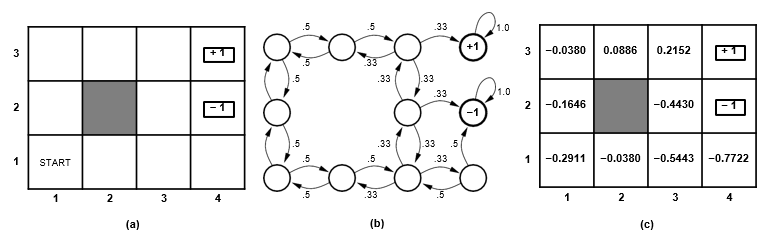
\includegraphics[width=\textwidth]{../out/images/value-function-example}
    \caption[value function example]{value function example}
    \label{fig:value function example}
\end{figure}

\section{Exploration and Delayed Reinforcement}\label{sec:exploration-and-delayed-reinforcement}

For small environments, we can compute the value function using simultaneous
equations.
For larger environments, we need a way of learning it, through experience.

\subsection{Exploration and delayed reinforcement}\label{subsec:exploration-and-delayed-reinforcement}

    I was born to try ...
    But you've got to make choices
    Be wrong or right
    Sometimes you've got to sacrifice the things you like.
    −\qquad-− Delta Goodrem

\subsection{Multi-Armed Bandit Problem}\label{subsec:multi-armed-bandit-problem}

\begin{figure}[h]
    \centering
    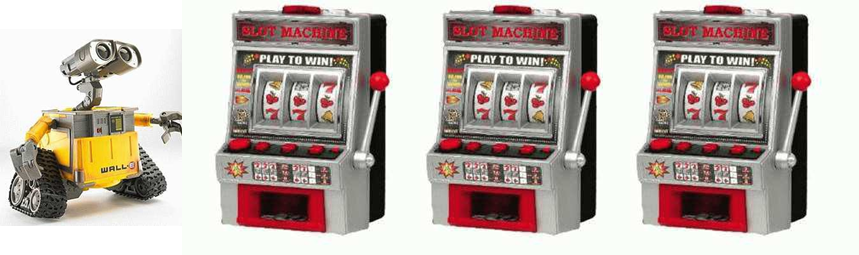
\includegraphics[width=\textwidth]{../out/images//multiarm_bandit}
    \caption[Multiarm Bandit]{multiarmbandit}
    \label{fig:multiarm_bandit}
\end{figure}

The special case of a stochastic reinforcement learning environment with only
one state is called the \textbb{Multi-Armed Bandit Problem}, because it is like being
in a room with several (friendly) slot machines (also called \("\)one-armed
bandits\("\)) for a limited time, and trying to collect as much money as
possible.
We assume that each slot machine provides rewards chosen from its own
(stationary) distribution, and that in each time step we are able to pull the
lever on only one machine.

\subsection{Exploration / Exploitation Tradeoff}\label{subsec:exploration-/-exploitation-tradeoff}
After pulling the levers a few times and observing the rewards received, it
makes sense that most of the time we should choose the lever (action) which we
think will give the highest expected reward, based on previous observations.

However, in order to ensure convergence to the optimal strategy, we must
occasionally choose something different from our preferred action.
Perhaps the simplest way to achieve this is known as an \textbb{epsilon-greedy
strategy}, where with probability $1 - \epsilon$ we choose what we think is the
best action, and with probability $\epsilon$ (typically, 5 percent) we choose
a random action.

\[P(a) = \dfrac{e^{R(a)/T}}{\sum_{b \in A^{R(b)/T}}}\]

More sophisticated strategies also exist such as Thompson Sampling, Upper
Confidence Bound (UCB) algorithms, or choosing from a Softmax (Boltzmann)
distribution based on the average reward so far observed for each action.

You may have noticed that we make the same kind of judgements about exploration
versus exploitation in everyday situations.
Should you eat at the old restaurant you have visited many times, or should you
try the newly opened restaurant across the street which might be worse but
might be much better?

\subsection{Optional video}\label{subsec:optional-video3}
insert video

\subsection{Delayed Reinforcement}\label{subsec:delayed-reinforcement}
The need for exploration also applies in the general case where there are
multiple states, and where we may need to take a whole sequence of actions in
order to get to the state from which we can obtain a high reward.

\begin{figure}[h]
    \centering
    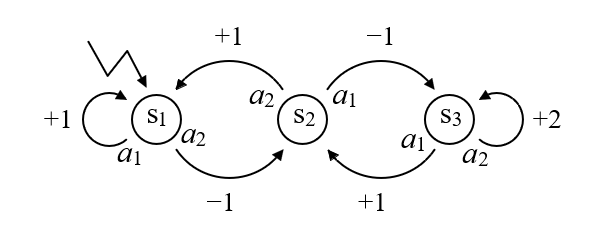
\includegraphics[width=\textwidth]{../out/images/asdf}
    \caption[asdf]{asdf}
    \label{fig:asdf}
\end{figure}

Recall that every policy $\pi$ determines a Value Function arrow
$V^{\pi}: S \to R$ where $V^{\pi}(s)$ is the expected discounted reward
received by an agent who begins in state sss and chooses its actions according
to policy $\pi$.

If $\pi = \pi^*$ is optimal, then $V^* (s) = V^{\pi^*}(s)$ is the maximum
(expected) discounted reward obtainable from state $s$.
Knowing this optimal value function can help to determine the optimal policy.

\subsection{Computing the Value Function}\label{subsec:computing-the-value-function}

Let $\gamma = 0.9$ and consider the policy $\pi : S_1 \mapsto a_2 , S_2 \mapsto a_1, S_3 \mapsto a_2$.
We have

\[
\begin{aligned}
V^{\pi} (S_3) &= \dfrac{2}{1 - \gamma} = 20 \\
V^{\pi}(S_2) &= -1 + \gamma V (S_3) = -1 + 18 = 17 \\
V^{\pi}(S_1) &= -1 + \gamma V (S_2) = -1 + 15.3 = 14.3
\end{aligned}
\]

For this example, the policy $\pi$ shown above must be the \textbb{optimal}
policy, because the value function for states $S_1$ and $S_2$ under any other
policy would not be more than 101010.
Therefore, the optimal value function is

\[V^* : S_1 \mapto 14.3, S_2 \mapsto 20\]

If we were given this value function $V^*$, we could use it to determine the
optimal policy $\pi$ provided we also know the reward function $R: S \times Z \to R$
and the transfer function $\delta : S \times A \to S$.
This information is sometimes called the \("\)World Model\("\).

\subsection{Video: Computing the Value Function}\label{subsec:video:-computing-the-value-function}
insert video

\subsection{Q-Function}\label{subsec:q-function}
The Q-function is a more sophisticated version of the value function which
enables an agent to act optimally without needing to know the World Model.
For any policy $\pi$, the \textbb{Q-function} $Q^{\pi} (s,a)$ is the expected
discounted reward received by an agent who begins in state $s$, first performs
action $a$ and then follows policy $\pi$ for all subsequent timesteps.

If $\pi = \pi^*$ is optimal, then $Q^* (s,a) = Q^{\pi^*}(s,a)$ is the maximum
(expected) discounted reward obtainable from sss, if the agent is forced to
take action aaa in the first timestep but can act optimally thereafter.

If the optimal Q-function $Q^*$ is known, then the optimal policy is given by

\[\pi^* (s) = \arg \max Q^* (s,a)\]

The Q-function for the environment shown above can be computed as follows:

\[
\begin{aligned}
    Q(S_1, a_1 ) &= 1 + \gamma V(S_1 ) = 1 + 0.9 \times 14.3 = 13.87 \\
    Q(S_1, a_2 ) &= V(S_1 ) = 14.3 \\
    Q(S_2, a_1 ) &= V(S_2) = 17 \\
    Q(S_2, a_2 ) &= 1 + \gamma V(S_1) = 13.87 \\
    Q(S_3, a_1 ) &= 1 + \gamma V(S_2) = 1 + 0.9 \times 17 = 16.3 \\
    Q(S_3, a_2 ) &= V(S_3) = 20
\end{aligned}
\]

\subsection{Optional video}\label{subsec:optional-video5}
insert video

\section{TD-learning and Q-learning}\label{sec:td-learning-and-q-learning}
Reinforcement Learning algorithms can generally be grouped into three classes:

\begin{itemize}
  \item Value function learning, including TD-Learning and Q-Learning
  \item Policy learning, including policy gradients and evolution strategies
  \item Actor-Critic, which is a combination of value function and policy learning
\end{itemize}

\subsection{Value Function Learning}\label{subsec:value-function-learning}
Recall that if $\pi = \pi^*$ is optimal, then $V^*(s) = V^{\pi^*} (s)$ is the
maximum (expected) discounted reward obtainable from state $s$, and
$Q^*(s,a) = Q^{\pi^*}(s,a)$ is the maximum (expected) discounted reward
obtainable from $s$, if the agent is forced to take action aaa in the first
timestep but can act optimally thereafter.

The idea behind value function learning is that the agent retains its own
estimate $V^*()$ or $Q^*()$ of the \("\)true\("\) value function $V^*()$ or $Q^*()$.
This estimate might be quite inaccurate to start with, but it gets iteratively
improved over time so that it more closely approximates the true value.
This process is sometimes called \("B\)ootstrapping\("\).

\subsection{Temporal Difference Learning}\label{subsec:temporal-difference-learning}
Let’s first assume that $R$ and $\delta$ are deterministic.
Then the (true) value $V*(s)$ of the current state $s$ should be equal to the
immediate reward plus the discounted value of the next state

\[V^*(s) = R(s,a) + \gamma V^* (\delta (s,a))\]

We can turn this into an update rule for the estimated value:

\[V(s_t) \leftarrow r_t + \gamma V (s_{t+1})\]

If $R$ and \delta$$ are stochastic (multi-valued), it is not safe to simply
replace $V(s)$ with the expression on the right hand side.
Instead, we move its value fractionally in this direction, proportional to a
learning rate $\eta$.

\[V(s_t) \leftarrow V(s_t) + \eta[r_t + \gamma V (s_{t + 1}) - V(s_{t})]\]

\subsection{Q-Learning}\label{subsec:q-learning}
Q-learning is similar to TD-learning except that the Q-function
$Q^*: S \times A \to R$ depends on a state, action pair instead of just a state.

For a deterministic environment, $\pi^*, Q^*$ and $V^*$ are related by

\[
\begin{aligned}
    \pi^* (s) &= \arg \max Q^* (s, a) \\
    Q^* (s,a) &= R(s,a) + \gamma V^* (\delta (s,a)) \\
    V^*(s) &= \max Q^* (s,b) \\
    \text{so} Q*(s,a) &= R(s,a) + \gamma \max Q^* (s,b)
\end{aligned}
\]

The last equation suggests that we can iteratively update our estimate by

\[Q (s_t , a_t ) \laftarrow r_t + \gamma \max Q (s_{t+1}, b)\]

If the environment is stochastic, we instead write

\[Q (s_t , a_t ) \laftarrow Q(s_t, a_t) + \eta [r_t + \gamma \max Q(s_{t+1}, b) - Q(s_t, a_t)]\]

\subsection{Optional video}\label{subsec:optional-video6}
insert video

\subsection{Theoretical Results and Generalization}\label{subsec:theoretical-results-and-generalization}
It can be proved that TD-learning and Q-learning will eventually converge to
the optimal policy, for any deterministic Markov decision process, assuming an
appropriately randomised strategy (Sutton, 1988; Watkins \& Dayan 1992; Dayan \& S
ejnowski, 1994).

However, these results rely on the assumption that every state will be visited
many times.
For small environments with a limited number of states and actions, this
assumption is reasonable.
For more challenging environments, the number of states can be exponentially
large, and it may be impractical to assume that every state will be visited even
once.
In these situations, we need to rely on a model such as a neural network that
is able to generalise to estimate the value of new states based on their
similarity with states that have previously been encountered.

\subsection{Optional video}\label{subsec:optional-video7}
insert video

\subsection{Computer Game Playing}\label{subsec:computer-game-playing}
Suppose we want to write a computer program to play a game like backgammon,
chess, checkers or Go. This can be done using a tree search algorithm
(expectimax, MCTS, or minimax with alpha-beta pruning).
But we need:

(a) an scheme for encoding any board position as a set of numbers, and
(b) a way to train a neural network or other learning system to compute a board evaluation, based on those numbers.

\subsection{Backgammon}\label{subsec:backgammon}

\begin{figure}[h]
    \centering
    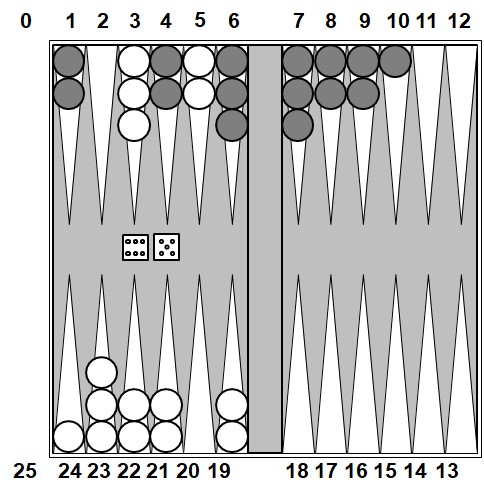
\includegraphics[width=\textwidth]{../out/images/backgammon}
    \caption[backgammon]{backgammon}
    \label{fig:backgammon}
\end{figure}

One of the first practical applications of TD-learning (Tesauro, 1992) was to
play the game of backgammon, which involves rolling dice and moving pieces
around a board with 24 \("\)points\("\).
In the above diagram, the white player is moving their pieces clockwise toward
the bottom left quadrant while the black player is moving their pieces
anti-clockwise toward the upper left quadrant.
When a player gets all of their pieces into the last quadrant, they can use the
dice rolls to move pieces off the board.
The first player to get all of their pieces off the board is the winner.

If a player has only one piece on a point (such as point 10 or 24 above) and
the other player moves a piece to that point, the original piece is sent back
to the \("\)bar\("\) and must start again from the beginning.
If a player has two or more pieces on a point, the other player is not allowed
to move a piece to that point.
We see in the above position that the black player has multiple pieces on
points 1, 4, 6, 7, 8, 9 so that the white player will not be able to move their
pieces on points 3 or 5 unless they roll either 2, 5 or 6.

\subsection{TD-Learning and Q-Learning}\label{subsec:td-learning-and-q-learning2}
One of the first practical applications of TD-learning (Tesauro, 1992) was to
play the game of backgammon, which involves rolling dice and moving pieces
around a board with 24 \("\)points\("\).
In the above diagram, the white player is moving their pieces clockwise toward
the bottom left quadrant while the black player is moving their pieces
anti-clockwise toward the upper left quadrant.
When a player gets all of their pieces into the last quadrant, they can use the
dice rolls to move pieces off the board.
The first player to get all of their pieces off the board is the winner.

If a player has only one piece on a point (such as point 10 or 24 above) and
the other player moves a piece to that point, the original piece is sent back
to the \("\)bar\("\) and must start again from the beginning.
If a player has two or more pieces on a point, the other player is not allowed
to move a piece to that point.
We see in the above position that the black player has multiple pieces on
points 1, 4, 6, 7, 8, 9 so that the white player will not be able to move their
pieces on points 3 or 5 unless they roll either 2, 5 or 6.

\subsection{TD-Gammon Neural Network}\label{subsec:td-gammon-neural-network}
TD-Gammon used a 2-layer neural network with 196 inputs, 20 hidden nodes and 1
output.
The inputs are arranged as follows:
\begin{itemize}
  \item 4 units × 2 players × 24 points
  \item 2 units for pieces on the bar
  \item 2 units for pieces off the board
\end{itemize}

Four inputs are assigned to each colour and each point, with a 1-hot encoding
used to specify one, two or three pieces and the fourth input scaled in
proportion to the number of pieces if there are more than three.
Additional inputs specify the number of pieces of each colour which are on the
bar, or off the board.

For any encoded board state, the network produces an output $V$ between 0 and
1 which is interpreted as its estimate of the probability of winning from that
state.

At each timestep, the dice are rolled, the network considers all possible legal
moves and computes the “next board position” that would result from each move.
These are converted to the appropriate input format, fed to the network, and
the one which produces the largest output is chosen.

The network can be trained by backpropagation using this formula
\[w_i \leftarrow w_i + \eta (T - V) \dfrac{\partial V}{\partial w_i}\]
where  are the weights in the network, $$ is the learning rate, $V$ is the
actual output of the network, and TTT is the target value.

The question is: How do we determine the target value $T$? In other words,
how do we know what the value of the current position \("\)should\("\) have been?
Alternatively, how do we find a better estimate for the value of the current position?

\subsection{How to choose the Target value}\label{subsec:how-to-choose-the-target-value}
One approach is to have a human expert play many games and build a database of
positions, dice rolls and chosen moves, similar to what was done for the ALVINN
autonomous driving system we discussed in Week 1.
The network could then be trained to increase the evaluation of each move
chosen by the human expert and decrease that of other moves which were
available but did not get chosen.

Another approach is for the network to learn from self-play by TD-learning,
effectively using the evaluation of subsequent positions in the game to refine
the evaluation of earlier positions.

Other methods such as TD-Root, TD-Leaf, MCTS and TreeStrap (Veness et al.,
2009) combine learning with tree search.
These are important for deterministic games like chess or Go, but less
important for a stochastic game like backgammon because the randomness of the
dice rolls limits the benefit of deep lookahead.

For backgammon, the agent receives just a single reward at the end of each
game, which we can consider as the final value  (typically, +1 for a win or -1
for a loss).
We then have a sequence of game positions, each with its own (estimated) value:

\[\text{(current estimate)} V_t \to V_{t+1} \to \dots \to V_m \to V_{m+1} \text{(final result)}\]

In this context, TD-learning simplifies and becomes equivalent to using the
value of the next state as the training value for the current state.
A fancier version, called TD, uses a weighted average over future estimates as
the training value for, where

\[T_k = (1 - \lambda) \sum_{k=t+1}^{m} \lambda^{k-1-t} V_k + \lambda^{m-t} V_{m+1}\]

The parameter $\lambda$ between 0 and 1 serves as a kind of discount factor,
but is different to the usual discount factor $\gamma$ (which can be equal to
$1$ in the case of TD-Gammon, because we do not care when we get the reward so
long as we get it).

\subsection{TD-Gammon}\label{subsec:td-gammon}
Tesauro trained two networks −-− one using Expert Preferences (EP), the other
by TD-learning (TD).
The TD-network outperformed the EP-network, and with modifications such as
3-step lookahead (expectimax) and additional hand-crafted input features,
became the best backgammon player in the world in 1995.

\subsection{Optional video}\label{subsec:optional-video8}
insert video

\subsection{Exercise: Reinforcement learning}\label{subsec:exercise:-reinforcement-learning}

Consider an environment with two states $S = \{\ S_1, S_2 \}\ $ and two actions
$A = \{\ a_1, a_2 \}\ $
where the deterministic transitions $\delta$ and reward $R$ for each state and
action are as follows:

\begin{figure}[H]
    \centering
    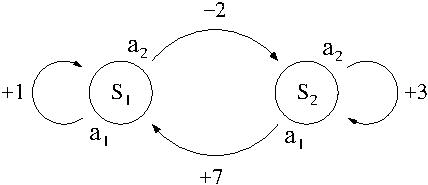
\includegraphics[width=\textwidth]{../out/images/question-1}
    \caption[question 1]{question 1}
    \label{fig:question 1}
\end{figure}

\[
\begin{aligned}
    \delta (S_1, a_1) &= s_1, R(S_1, a_1) = +1 \\
    \delta (S_1, a_2) &= s_2, R(S_1, a_2) = -2 \\
    \delta (S_2, a_1) &= s_1, R(S_2, a_1) = +7 \\
    \delta (S_2, a_2) &= s_2, R(S_2, a_2) = +3 \\
\end{aligned}
\]

\textbf{question 1}
Assuming a discount factor of $\gamma = 0.7$, determine the optimal policy
$\pi^* : S \to A$

\textbf{Answer}
\[
\begin{aligned}
\pi^* (S_1) &= a_2 \\
\pi^* (S_2) &= a_1 \\
\end{aligned}
\]

\textbf{Question 2}
Still assuming $\gamma = 0.7$ determine the value function $V: S \\to R$

\textbf{Answer}
\[
\begin{aligned}
    V(S_1) &= 5.69 \\
    V(S_2) &= 10.98 \\
\end{aligned}
\]

\textbf{Explanation}
\[
\begin{aligned}
V(S_1) &= -2 + \gamma V(S_2) \\
V(S_2) &= +7 + \gamma V(S_1) \\
\text{So} V(S_1) &= -2 + 7 \gamma + \gamma^2 V(S_1) \\
\text{i.e.} V(S_1) &= \dfrac{-2 + 7\gamma}{1 - \gamma^2} = \dfrac{-2 + 7 \times 0.7}{1 - 0.49} = 5.69 \\
\text{Then} V(S_2) &= 7 + 0.7 \times 5.69 = 10.98\\
\end{aligned}
\]

\textbf{Question 3}
still assuming $\gamma = 0.7$, determine the values of the Q-function
$Q: S \times A \to R$

\textbf{Answer}
\[
\begin{aligned}
Q(S_1, a_1) &= 1 + \gamma V (S_1) &= 4.98 \\
Q(S_1, a_2) &= V(S_1) &= 5.69 \\
Q(S_2, a_1) &= V(S_2) &= 10.98 \\
Q(S_2, a_2) &= 3 + \gamma V(S_2) &= 10.69 \\
\end{aligned}
\]

\textbf{Question 4}
Still assuming $\gamma = 0.7$, trace through the first few steps of the
Q-learning algorithm, assuming a learning rate of 1 and with all Q values
initially set to zero.
Explain why it is necessary to force exploration through probabilistic choice
of actions, in order to ensure convergence to the true Q values.

Here are some hints to get you started:

Since the learning rate is 1 (and the environment deterministic) we can use
this Q-Learning update rule:

\[Q(S,a) \leftarrow r(S,a) + \gamma \max Q(\delta(S,a),b)\]

Let's assume the agent starts in state $S_1$.
Because the initial Q values are all zero, the first action must be chosen randomly.
If action  is chosen, the agent will get a reward of +1 and the update will be

\[Q(S_1, a_1) \leftarrow 1 + \gamma \times 0 = 1\]

\textbf{Answer}
With a deterministic environment and a learning rate of 1, the Q-learning update rule is
\[Q(S,a) \leftarrow r(S,a) + \gamma \max Q(\delta(S,a),b)\]

if the agent starts in a state $S_1$ and chooses action $a_1$, it will get a reward of +1 and the update will be:

\[Q(S_1, a_1) \leftarrow 1 + \gamma \times 0 = 1\]

we do \textbf{not} force exploration, the agent will always prefer action $a_1$
in state $S_1$, and will never explore action $a_2$ this means that $Q(S_1, a_2)$
will remain zero forever, instead of converging to the true value of 5.69.
If we \textbf{do} force exploration, the next steps may look like this:

\begin{center}
\begin{tabular}{ c c c }
 current state & chosen state & new Q value \\
 $cell4S_1$ & $cell5a_2$ & $-2 + \gamma \times = -2$ \\
 $S_2$ & $a_2$ & $3 + \gamma \times 0 = 3$
\end{tabular}
\end{center}

At this point the table looks like this:

\begin{center}
\begin{tabular}{ c c c }
 Q & $a_1$ & $a_2$ \\
 $S_1$ & 1 & -2 \\
 $cell7S_2$ & 0 & 3
\end{tabular}
\end{center}

Again we need to force exploration in order to the get the agent to choose $a_1$
from $S_2$ and to again choose $a_2$ from $S_1$

\begin{center}
\begin{tabular}{ c c c }
 current state & chosen action & new Q value \\
 $cell4S_2$ & $a_1$ & $7 + \gamma \times 1 = 7.7$ \\
 $S_1$ & $a_2$ & $-2 + \gamma 7.7 = 3.39$
\end{tabular}
\end{center}

\begin{center}
\begin{tabular}{ c c c }
 Q & $a_1$ & $a_2$ \\
 $S_1$ & 1 & 3.39 \\
 $S_2$ & 7.7 & 3
\end{tabular}
\end{center}

Further steps will refine the Q value estimates, and in the limit they will
converge to their true values

\textbf{Question 5}
Now let's consider how the value function changes as the discount factor $\gamma$
varies between 0 and 1.
There are four deterministic policies for this environment, which can be
written as $\pi_{11}, \pi_{12}, \pi_{21}$, and $\pi_{22}$, where
$\pi_{ij} (S_1) = a_1, \pi_{ij}(S_2) = a_j$

Calculate the value function $V_{(\gamma)}^{\pi}: S \to R$ for each of these
four policies (keeping $\gamma$ as a variable)

\textbf{Answer}
\begin{figure}[h]
    \centering
    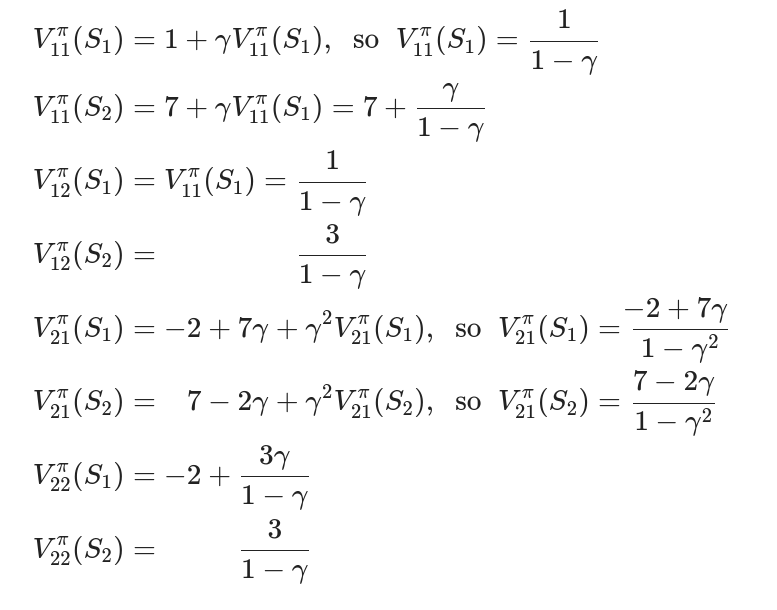
\includegraphics[width=\textwidth]{../out/images/5a_5}
    \caption[5a\_5]{5a\_5}
    \label{fig:5a_5}
\end{figure}

\textbf{Question 6}
Determine for which range of values $\gamma$ each of the policies
$\pi_{11}, \pi_{12}, \pi_{21}, \pi_{22}$ is optimal

\textbf{Answer}
$\pi_{11}$ is optimal when:
\[0 < V_{11}^{\pi}(S_1) - V_{21}^{\pi} (S_1) = \dfrac{(1+\gamma) - (-2 + 7\gamma)}{1 - \gamma^2} = \dfrac{3 - 6\gamma}{1 - \gamma^2} \text{i.e.} 0 \leq \gamma \leq 0.5\]

$\pi_{22}$ is optimal when

\[0 < V_{22}^{\pi}(S_2) - V_{21}^{\pi} (S_2) = \dfrac{3(1 + \gamma) - (7 - 2\gamma)}{1 - \gamma^2} = \dfrac{-4 + 5\gamma}{1 - \gamma^2} \text{i.e.} 0.8 \leq \gamma \leq 1.0\]

$\pi_{21}$ is optimal for $0.5 \leq \gamma \leq 0.8$

$\pi_{12}$ is never optimal because it is dominated by $\pi_{11}$ when $\gamma < 2/3$ and by $\pi_{22}$ when $\gamma > 0.6$

\subsection{Exercise: Reinforcement Learning}\label{subsec:exercise:-reinforcement-learning2}
This is a revision quiz to test your understanding of the material from Week 5 on Reinforcement Learning.

You must attempt to answer each question yourself, before looking at the sample answer.

\textbf{Question 1}
Describe the elements (sets and functions) that are needed to give a formal
description of a reinforcement learning environment.
What is the difference between a deterministic environment and a stochastic
environment?

\textbf{Answer}
Formally, a reinforcement learning environment is defined by a set of
$\mathcal{S}$ states, a set of $\mathcal{A}$, a transition function $\delta$
and a reward function $\mathcal{R}$

For a stochastic environment $\delta$ and $\mathcal{R}$ are single-valued functions:
\[
\begin{aligned}
    \delta : \mathcal{S} \times \mathcal{A} \to \mathcal{S} \\
    \mathcal{R}: \mathcal{S} \times \mathcal{A} \to \mathbb{R}
\end{aligned}
\]

For a stochastic environment $\delta$ and/or $\mathcal{R}$ are not
single-valued, but instead define a probability distribution on $\mathcal{S}$
or $\mathbb{R}$

\textbf{Question 2}
Name three different models of optimality in reinforcement learning, and give
a formula for calculating each one.

\textbf{Answer}
\[
\begin{aligned}
    \text{Finite horizon reward} &: \sum_{i=0}^{h-1} r_{t+i} \\
    \text{Infinite discounted reward} &: \sum_{i=0}^{\infty} \gamma^i r_{t+i}, 0 \leq \gamma < 1 \\
    \text{Average reward} &: \lim_{h \to \infty} \dfrac{1}{h} \sum_{h-1}^{i=0} r_{t+i}
\end{aligned}
\]

\textbf{Question 3}
What is the definition of:
\begin{itemize}
    \item the optimal policy
    \item the value function
    \item the Q-function?
\end{itemize}

\textbf{Answer}
the optimal policy is the function $\pi^* : \mathcal{S} \to \mathcal{A}$ which maximises the infinite discounted reward.

the value function $V^{\pi}(S)$ is the expected infinite discounted reward
received by an agent who begins in state $s$, first performs action $a$ and
then $V^*(s) = V^{\pi^*}(s)$ is the maximum (expected) infinite discounted
reward obtainable from state $s$

The Q-function $Q^{\pi}(spa)$ is the expected infinite discounted reward
received by an agent who begins in state $s$, first performs action $a$ and
then follows policy $\pi$ for all subsequent timesteps If $\pi = \pi^*$ is
optimal, then $Q^*(s,a) = Q^{\pi}^* (s,a)$ is the maximum (expected) discounted
reward obtainable from $s$ if the agent is forced to take action $a$ in the
first time step but can act optimally thereafter.

\textbf{Question 4}
Assuming a stochastic environment, discount factor $\gamma$ and learning rate
of $\eta$, write the equation for
\begin{itemize}
    \item Temporal Difference learning TD(0)
    \item Q-Learning
\end{itemize}
Remember to define any symbols you use.

\textbf{Answer}
\begin{gather*}
    V(s_t) \leftarrow V(s_t) + \eta [r_t + \gamma V (s_{t + 1}) - V(s_{t})]\\
    Q(s_t, a_t ) \leftarrow Q(s_t a_t) + \eta [r_t + \gamma \max_b Q(s_{t+1}, b)- Q(s_t, a_t)]\\
    s_t = \text{ state at time } t, a_t = \text{ action performed at time} t, \\
    r_t = \text{ reward received at time }t, s_{t+1} = \text{ state at time } t + 1 \\
\end{gather*}

\part{Policy Learning and Deep RL}\label{part:policy-learning-and-deep-rl}

\section{Policy Learning}\label{sec:policy-learning}
Policy learning algorithms do not use a value function but instead operate
directly on the policy, chosen from a family of policies
$\pi_{\theta}: S \mapto A$ determined by parameters $\theta$.

Typically, $\pi_{\theta}$ is a neural network with weights $\theta$ which takes
a state $s$ as input and produces action $a$ as output, which may be either
continuous or discrete.

If there is a discrete choice of actions, the network has one output for each
possible action and uses Softmax to determine the conditional probability  of
performing action $a$ in state $s$.

For episodic domains like Backgammon, we do not need a discount factor, and the
\("\)fitness\("\) of policy $\pi_{\theta}$ can be taken as the Value function of the initial
states $s_0$ under this policy, which is the expected (or average) total reward
received in each game by an agent using policy $\pi_{\theta}$.

\[\text{fitness}(\pi_{\theta}) = V^{\pi \theta}(s_0) = E_{\pi \theta} (r_{\text{total}})\]

Policy Learning algorithms include Policy Gradients, which use gradient descent
to modify the parameters $$, and Evolution Strategies, which make random changes
to  and keep only those updates that are seen to increase the reward.

\section{Deep Reinforcement Learning}\label{sec:deep-reinforcement-learning}
\subsection{Deep Reinforcement Learning}\label{subsec:deep-reinforcement-learning}
\subsection{Deep Q-Learning for Atari Games}\label{subsec:deep-q-learning-for-atari-games}

Mnih (2015) demonstrated how Q-learning could be combined with deep CNNs to
learn to play Atari games from pixels.

\begin{figure}[H]
    \centering
    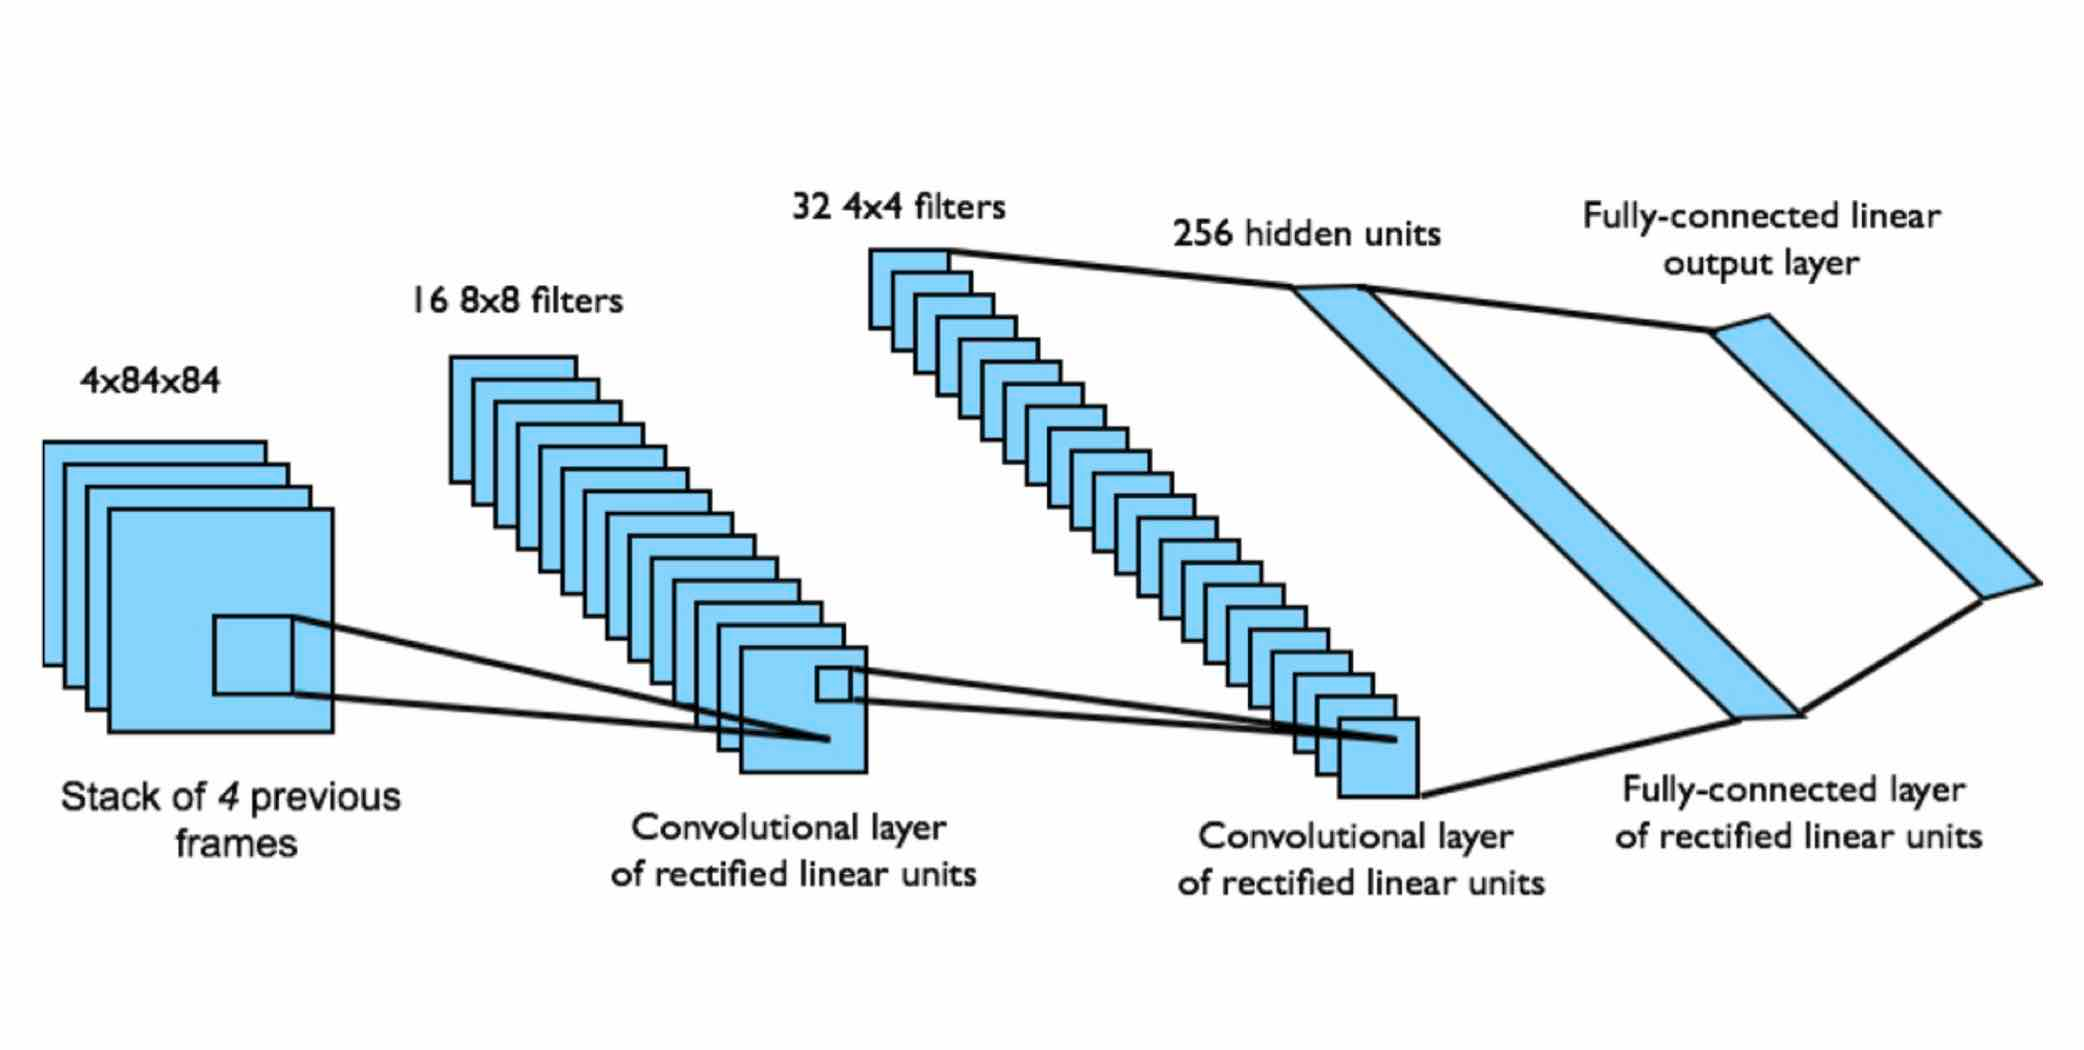
\includegraphics[width=\textwidth]{../out/images/atari-games}
    \caption[atari games]{atari games}
    \label{fig:atari games}
\end{figure}

The input state $s$ is a stack of raw pixels from four consecutive frames.
The images are converted from 8-bit RGB images at resolution $210 \times 160$
pixels to $84 \times 84$ greyscale images.
The 18 outputs are the Q-values $Q(s,a)$ for 18 different combinations of
joystick/button positions.
The reward is the change in score during the timestep.

\begin{figure}[H]
    \centering
    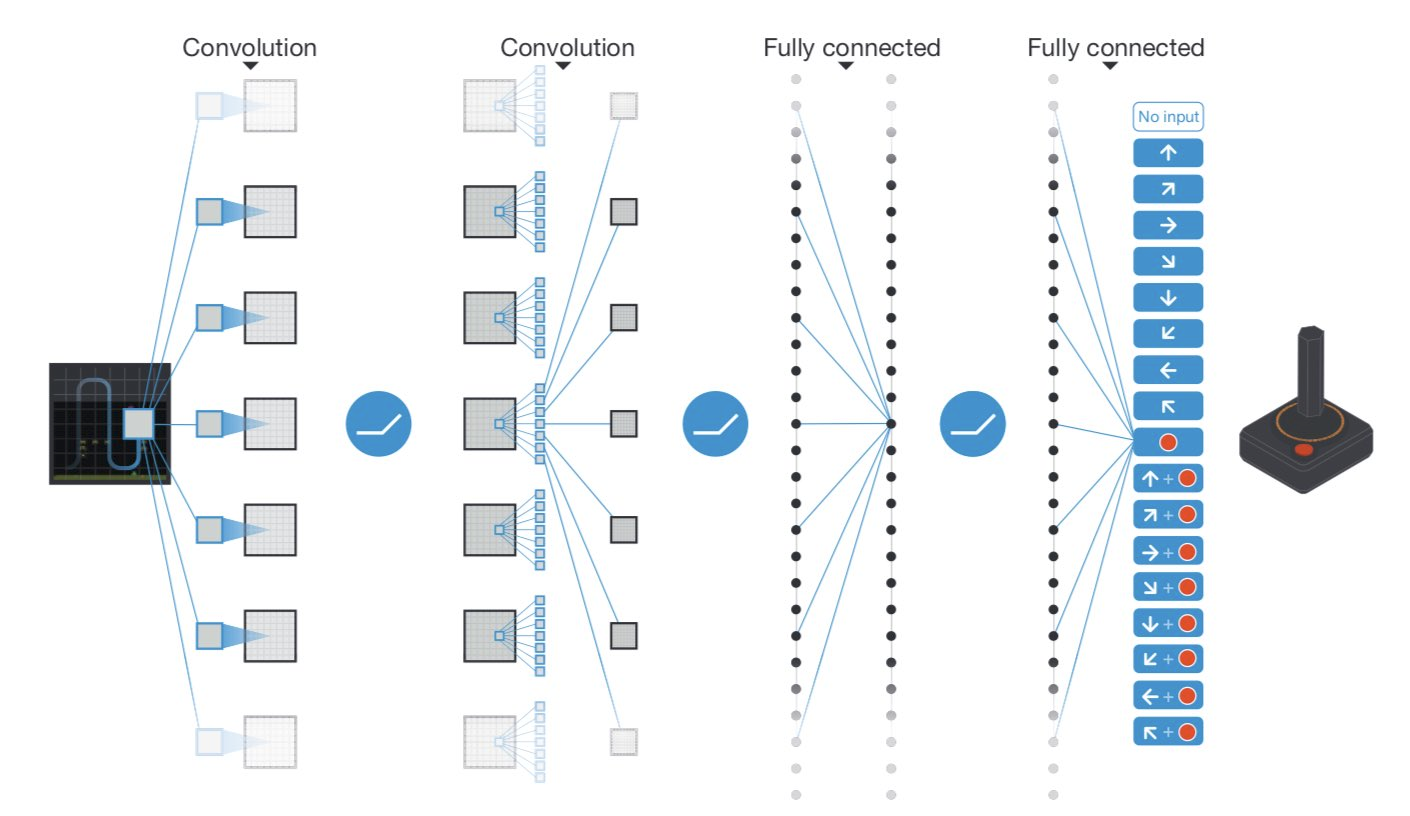
\includegraphics[width=\textwidth]{../out/images/deep-q-learning}
    \caption[deep q learning]{deep q learning}
    \label{fig:deep q learning}
\end{figure}
Recall the Q-Learning update rule:

\[Q(s_t, a_t ) \leftarrow Q(s_t, a_t ) + \eta \bigg[ r_t + \gamma \max Q(s_{t+1}, b) - Q(s_t,a_t)\bigg]\]

If a lookup table is used to store the Q values for every state and action
separately, the algorithm is guaranteed to eventually converge to an optimal
policy.
But, if the number of states is exponentially large, we must instead use a
neural network $Q_w$ and adjust the weights www according to the Q-Learning update
rule, which is equivalent to minimizing:

\[\Bigg[ r_t + \gamma \max Q_w (s_{t+1}, b) - Q_w (s_i, a_t) \Bigg]^2\]

The gradient is applied only to $Q_w (s_t, a_t)$, \textbb{not} to $Q_w (s_{t+1}, b)$.

\section{Experience Replay}\label{sec:experience-replay}
Training of deep neural networks for classification tasks generally requires
that each mini-batch should include a variety of different inputs and target
outputs.
For Atari games, many similar states may occur in succession, often with the
same action being selected.
We can remove this \textbf{temporal} correlation between samples by storing
experiences in a Replay Buffer.

In this scenario, one thread repeatedly plays the game, selecting its actions
using an $\epsilon$-greedy strategy based on the current $\epsilon$-values, and
builds a database of experiences $s_t, a_t, r_t, s_{t+1}$.
Another thread samples asynchronously from this database and applies the
Q-learning rule to minimize

\[\Bigg[ r_t + \gamma \max Q_w (s_{t+1}, b) - Q_w (s_t, a_t) \Bigg]^2\]

This removes temporal correlations by sampling from a variety of game
situations in random order, and also makes it easier to parallelize the
algorithm on multiple GPUs.

\section{Optional video}\label{sec:optional-video11}

\section{Prioritised Replay}\label{sec:prioritised-replay}
Instead of sampling experiences uniformly, it may be more efficient to store
and retrieve them in a priority queue with priority based on the DQN error (Schaul, 2015).
\[|r_t + \gamma \max Qw(s_{t+1}, b) - Q_w (s_t, a_t)|\]

This ensures the system will concentrate more effort on situations where the
value was \("\)surprising\("\) (in the sense of being far away from what was predicted).

\section{Double Q-Learning}\label{sec:double-q-learning}
If the same weights www are used to select actions and to evaluate actions (as
well as states) the network may learn a suboptimal strategy due to a kind of
\("\)confirmation bias\("\).
One way to avoid this is to maintain two sets of weights www and , with one
used for action selection and the other for evaluation (then swap their roles).

In the context of Deep Q-learning, a simpler approach is to use the current
\("\)online\("\) version of www for selection, and an older \("\)target\("\)
version for evaluation (Van Hasselt, 2016).
We therefore minimize

A new version of is periodically calculated from the distributed values of $$ and
this $$ is broadcast to all processors.

\section{Advantage Function}\label{sec:advantage-function}

The  Function  can be written as a sum of the value function  plus an advantage function
 represents the advantage (or disadvantage) of taking action aaa in state $s$,
compared to taking the action preferred by the current policy .
We can learn approximations for these two components separately:

\[\]

Note that actions can be selected just using , because

\section{Optional video}\label{sec:optional-video10}

\subsection{Advantage Actor-Critic}\label{subsec:advantage-actor-critic}
Recall that in the REINFORCE algorithm, a baseline bbb could be subtracted from
for the purpose of variance reduction.

In the actor-critic framework,

We can also subtract a baseline from .
This baseline must be independent of the action at, , but it could be dependent on the state .
A good choice of baseline is the value function , in which case the Q function is replaced by the advantage function

\subsection{Asynchronous Advantage Actor-Critic}\label{subsec:asynchronous-advantage-actor-critic}

The Asynchronous Advantage Actor-Critic or  Algorithm combines a policy network , a value function network and an (estimated) Q-function.
\begin{itemize}
    \item use polity network  to choose actions
    \item learn a parameterised value function (s) by TD-learning
    \item estimate Q-value by n-step sample
    \item update policy  by
    \item update value function  by minimising
\end{itemize}

\subsection{Optional video}\label{subsec:optional-video9}

\section{Examples of Deep Reinforcement Learning}\label{sec:examples-of-deep-reinforcement-learning}

\end{document}